\chapter{Internship Experience}
\label{ch:internship_experience}

\section{Internship Achievements and Contributions}
\label{sec:internship_experience:achievements_contributions}

During my internship, I had the opportunity to contribute to various aspects of the application's development and functionality. I was able to implement several key features that enhanced the application's efficiency, security, and user experience. Below are the major contributions I made during my internship:

\subsection{ORM (Object-Relational Mapper)}
\label{subsec:internship_experience:orm}

We use SQLAlchemy as the ORM to define the models in Python. By using an ORM, we can define the models in Python like a normal class, and the ORM will take care of creating the database schema. This saves us time and effort, and allows us to focus on the business logic without having to worry about the database schema and lots of complex SQL queries~\cite{noauthor_sqlalchemy_nodate}.

\subsection{Base Models}
\label{subsec:internship_experience:base_models}

In our reporting application, several tables will be needed to store and manage data effectively.

\begin{itemize}
    \item \textbf{User:} This table will store information about the users of the application. Each user will have one or more roles assigned to them.
    \item \textbf{Role:} Since users can have multiple roles (e.g., Admin, Technician), a separate Role table will be used. This approach avoids embedding roles directly within the User table and allows for flexible role assignments.
    \item \textbf{POI (Point of Interest):} This table will store information about the places, objects, or conditions that users report. The POI can be quite abstract and represent various entities.
    \item \textbf{Status:} When a user reports an issue with a POI, the status of the report needs to be tracked. This table will store the different statuses a report can have. It will have an OPEN or CLOSED state, to indicate whether the report is still open or has been resolved.
    \item \textbf{Criticality:} To determine the urgency or importance of a status, a Criticality table will be used. This table will serve as a reference for how critical each status is.
\end{itemize}

These are the minimum tables needed to manage the application effectively. Additional tables will be also created to accomodate more features below.

\subsection{Managing Point of Interest Hierarchically}
\label{subsec:internship_experience:managing_poi}

Effectively monitoring a large number of POIs can be challenging. To address this, we use a hierarchical structure that organizes POIs into areas, and areas into regions. This approach simplifies identifying troubled POIs and allows for efficient management.

\begin{itemize}
    \item \textbf{Region:} This is the highest level, representing a broad area (e.g., Building A, Building B). It serves as a high-level overview and provides context for lower levels.
    \item \textbf{Area:} This level represents a subdivision within a region (e.g., Floor 1, Floor 2, etc.). It allows for a more focused analysis compared to the region level.
    \item \textbf{POI:} This is the lowest level, representing individual locations of interest (e.g., Main lobby, Parking area, etc). It provides the most granular details about a specific location.
\end{itemize}

This hierarchical structure offers several benefits:

\begin{itemize}
    \item \textbf{Efficient Management:} By breaking down the monitoring process into manageable levels, it becomes easier to identify and address issues at specific points, areas, or regions, leading to more effective management.
    \item \textbf{Simplified Reporting:}  The hierarchical structure facilitates clearer and more structured reporting, as information can be aggregated and summarized at different levels.
    \item \textbf{Scalability:} As the number of POIs increases, the hierarchical model can easily accommodate new entries without overwhelming the application, allowing for efficient scaling.
\end{itemize}

\subsection{Dynamic Reporting Forms}
\label{subsec:internship_experience:dynamic_reporting_forms}

To accommodate the varying information required in user's reports, we use \href{https://jsonforms.io/}{JSONForms} library to create dynamic forms based on predefined templates for each POI\@. This approach ensures that the reporting process is both flexible and tailored to the specific needs of different POIs.

\subsection{Access Control Level}
\label{subsec:internship_experience:access_control_level}

To maintain security and focus within the application, an access control level is implemented. This feature restricts users to accessing and reporting only on specific POIs assigned to them. By enforcing this restriction, users can concentrate on their designated areas of responsibility without being overwhelmed by the entire application. This approach ensures that access is managed effectively, promoting both security and efficiency throughout the platform.

\subsection{Group}
\label{subsec:internship_experience:group}

As the application grows, managing users can become challenging, especially when administrators need to manage access control for each user and their respective POIs. To facilitate easier user management, we use a grouping system. Administrators can group users together and assign these groups to specific POIs at the access control level. This approach allows administrators to manage the access control of multiple users simultaneously.

\subsection{Communication}
\label{subsec:internship_experience:communication}

Effective communication is essential for users to discuss issues, share information, and collaborate on problem-solving. To facilitate this, a real-time group chat feature is implemented at the Area level. This feature allows users to engage in discussions, share information, and collaborate more effectively. It provides a centralized platform for communication, reducing the need for multiple tools and ensuring that all relevant parties are kept informed.

Additionally, a Notification feature is implemented, enabling administrators to send important messages to all or specific users and groups. This ensures timely dissemination of critical information.

A Comment feature is also available, allowing users to comment on specific statuses. This helps users provide additional information, ask questions, or give feedback on particular issues, enhancing overall communication and collaboration.

\subsection{Audit}
\label{subsec:internship_experience:audit}

As administrators overseeing the situation via the dashboard, it is crucial not only to review statuses from POIs but also to monitor changes occurring within the application. To achieve this, an audit trail is implemented to capture all database-level changes. This comprehensive tracking allows for detailed analysis and provides valuable insights into user activity, data modifications, and application performance. An event listener from SQLAlchemy provides an efficient way to log changes automatically.

\subsection{Real-time data and notifications}
\label{subsec:internship_experience:realtime_data_notifications}

To enhance data visualization on the dashboard, real-time data is required, such as current open statuses and critical statuses. To achieve this, Socket.IO is used to send data to the frontend in real-time, eliminating the need to refresh the page. By leveraging the audit log, notifications can also be sent to users when specific events occur, such as a new report or a status change. This ensures that users are promptly informed of important updates, improving overall responsiveness and user experience.

\subsection{User interface}
\label{subsec:internship_experience:user_interface}

User interface plays a critical role in ensuring that users can interact with the application effectively. Using React as the frontend library and Mantine as the UI framework, we can easily and quickly create a user-friendly interface that meets the needs of the users. We also need the user interface to be responsive, allowing users to access the application from different devices and screen sizes. Fortunately, Mantine provides a wide range of components that are responsive by default.

These are several key functionalities that the user interface should provide:

\begin{itemize}
    \item \textbf{Navbar and Header:} The navbar and header provide users with easy access to essential features such as reporting, notifications, and a way to navigate between different sections of the application. Not to forget the logo of the application and user profile.
    \item \textbf{Theme:} The theme of the application should be consistent and visually appealing. By using Mantine, we can easily customize the color palette, typography, and other design elements to create a cohesive and attractive interface. As we also want to configure the theme dynamically, we will store the theme settings in the database and allow different companies that leverage the application to customize the theme according to their branding.
    \item \textbf{Dashboard:} The central hub of the UI for the administrators. The dashboard provides admins with an overview of critical information such as current open statuses, notifications, and data visualizations. It allows users to quickly assess the status of POIs, areas, and regions at a glance.
    \item \textbf{Map:} The map view provides a visual representation of the POIs, areas, and regions. It allows users to see the geographical distribution of the POIs and their respective statuses. This map will be shown on the dashboard and can be interacted with to view more details.
    \item \textbf{Browse:} In browse, the users can view the list of POIs and their respective statuses. It also allows users to filter and search for specific POIs using name, and group the POIs by region or area.
    \item \textbf{Settings:} The settings page provides users with a table-like view of all the regions, areas, POIs, and other relevant entities. It allows users to manage and configure these entities effectively.
    \item \textbf{Users:} The users page allows administrators to manage users, groups, and roles. It provides a centralized platform for user management, access control, and role assignments.
    \item \textbf{Chat:} The chat page utilizes a real-time chat feature that allows users to engage in discussions, share information, and collaborate more effectively.
   
\end{itemize}

\section{Integration with External Services}
\label{sec:internship_experience:integration_external_services}

Now that the functionalities within the application are implemented, we are ready to integrate the app with external services. This will allow us to enrich the data and provide more value to the users. In this case, we are going to integrate weather data from \href{https://www.dwd.de/DE/Home/home_node.html}{Deutsche Wetterdienst (DWD)} to provide real-time weather information. We will create a POI called Frankfurt Weather' in the app. Then, using the message-oriented middleware Apache Camel, we will retrieve data from DWD using their REST API, process it, and forward the data through a REST API to the OpsEdge application. To make it easier to update a status for a POI, we will use the shortname' attribute in the POI model and create an endpoint for this, so that we do not have to use the ID of the POI every time we want to update its status externally.

\section{Pictures}
\label{sec:internship_experience:pictures}

\begin{figure}[h]
    \centering
    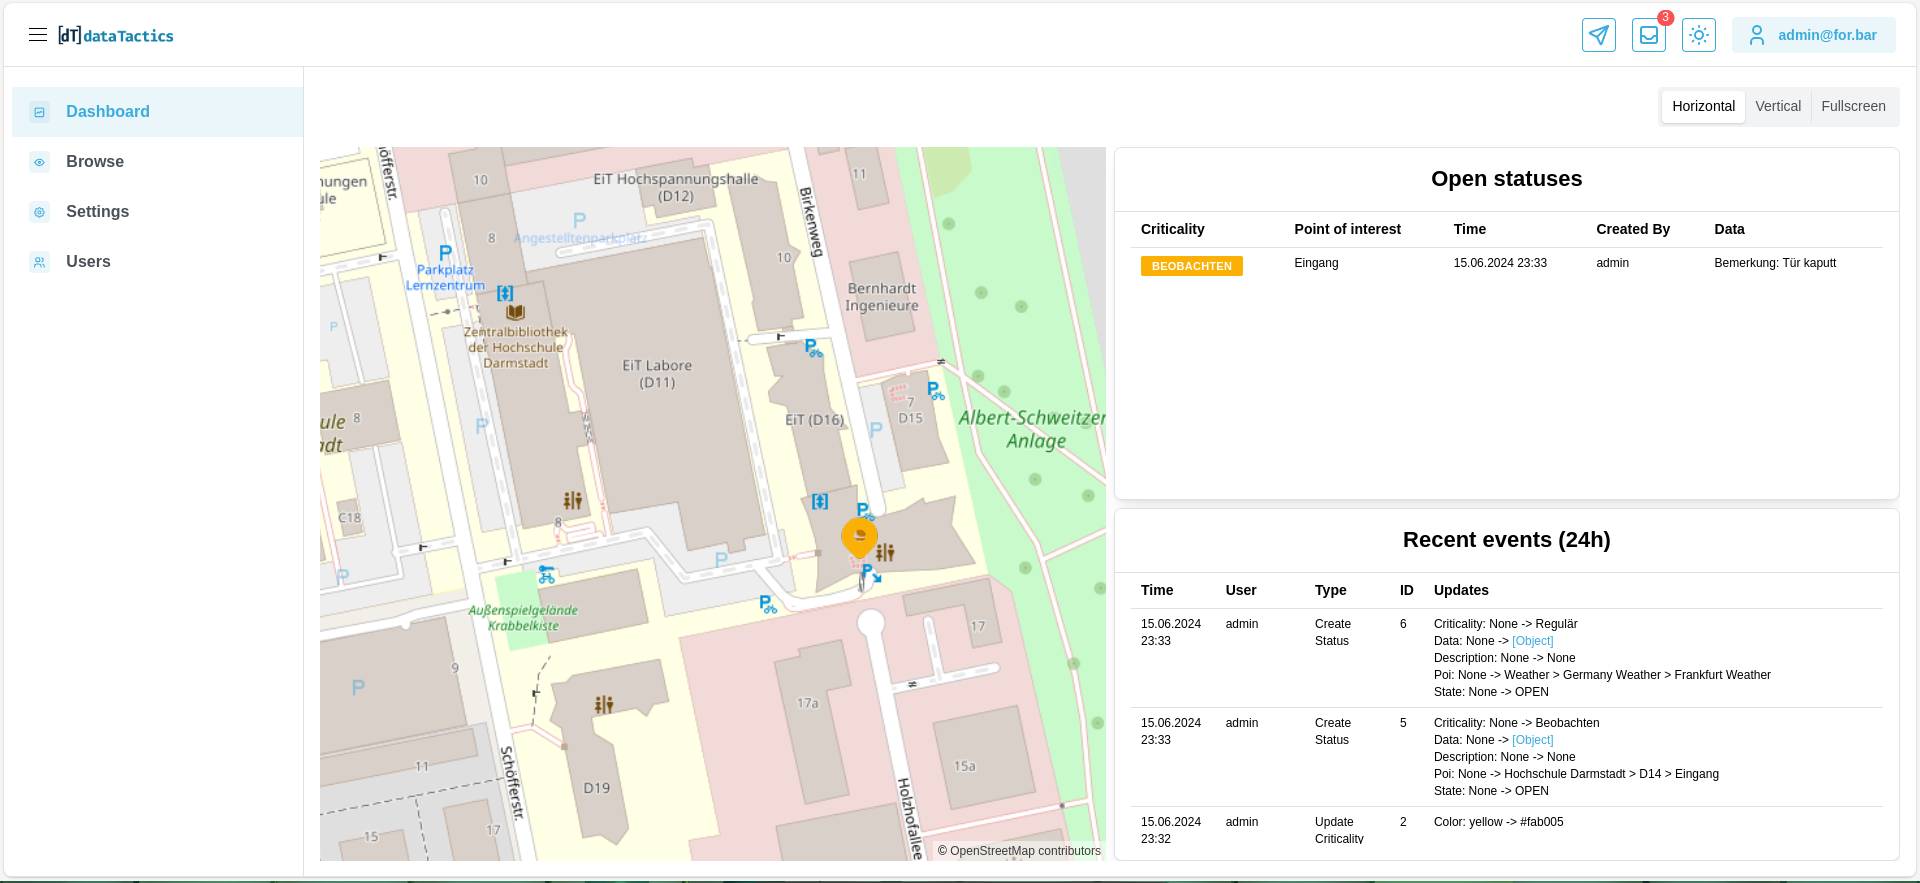
\includegraphics[width=1\textwidth]{gfx/opsedge-dashboard.png}
    \caption{OpsEdge Dashboard}
    \label{fig:opsedge_dashboard}
\end{figure}

\begin{figure}[h]
    \centering
    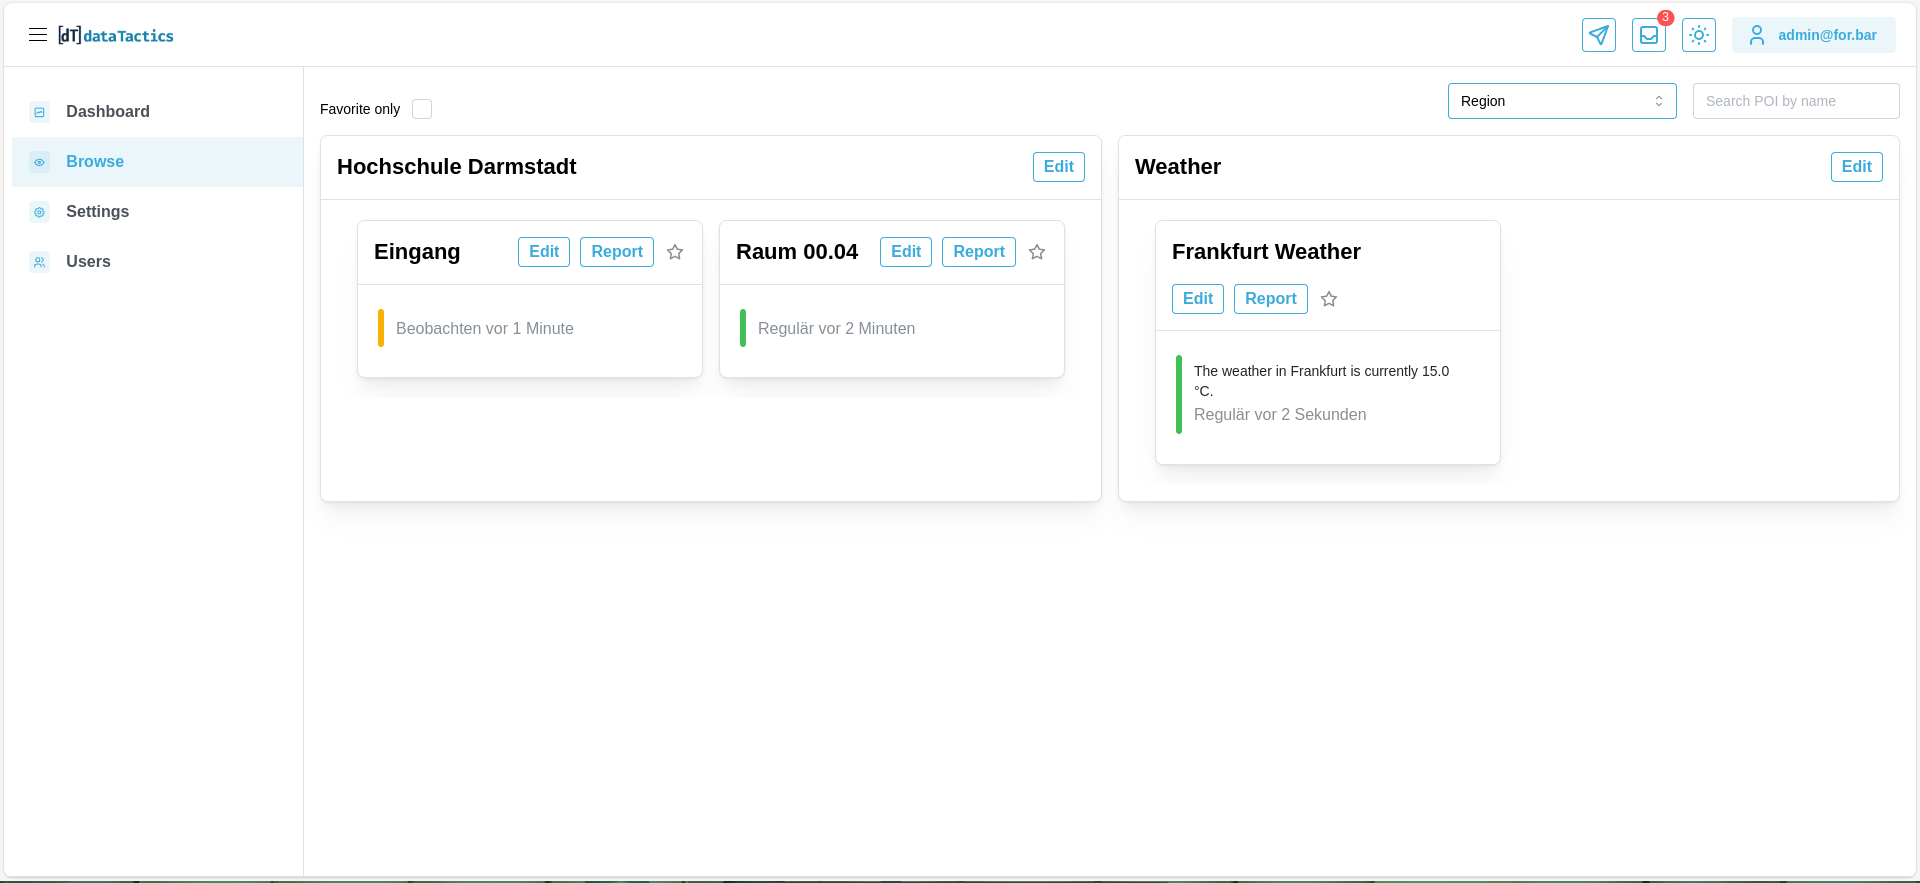
\includegraphics[width=1\textwidth]{gfx/opsedge-browse-group-by-region.png}
    \caption{OpsEdge Browse}
    \label{fig:opsedge_browse}
\end{figure}

\begin{figure}[h]
    \centering
    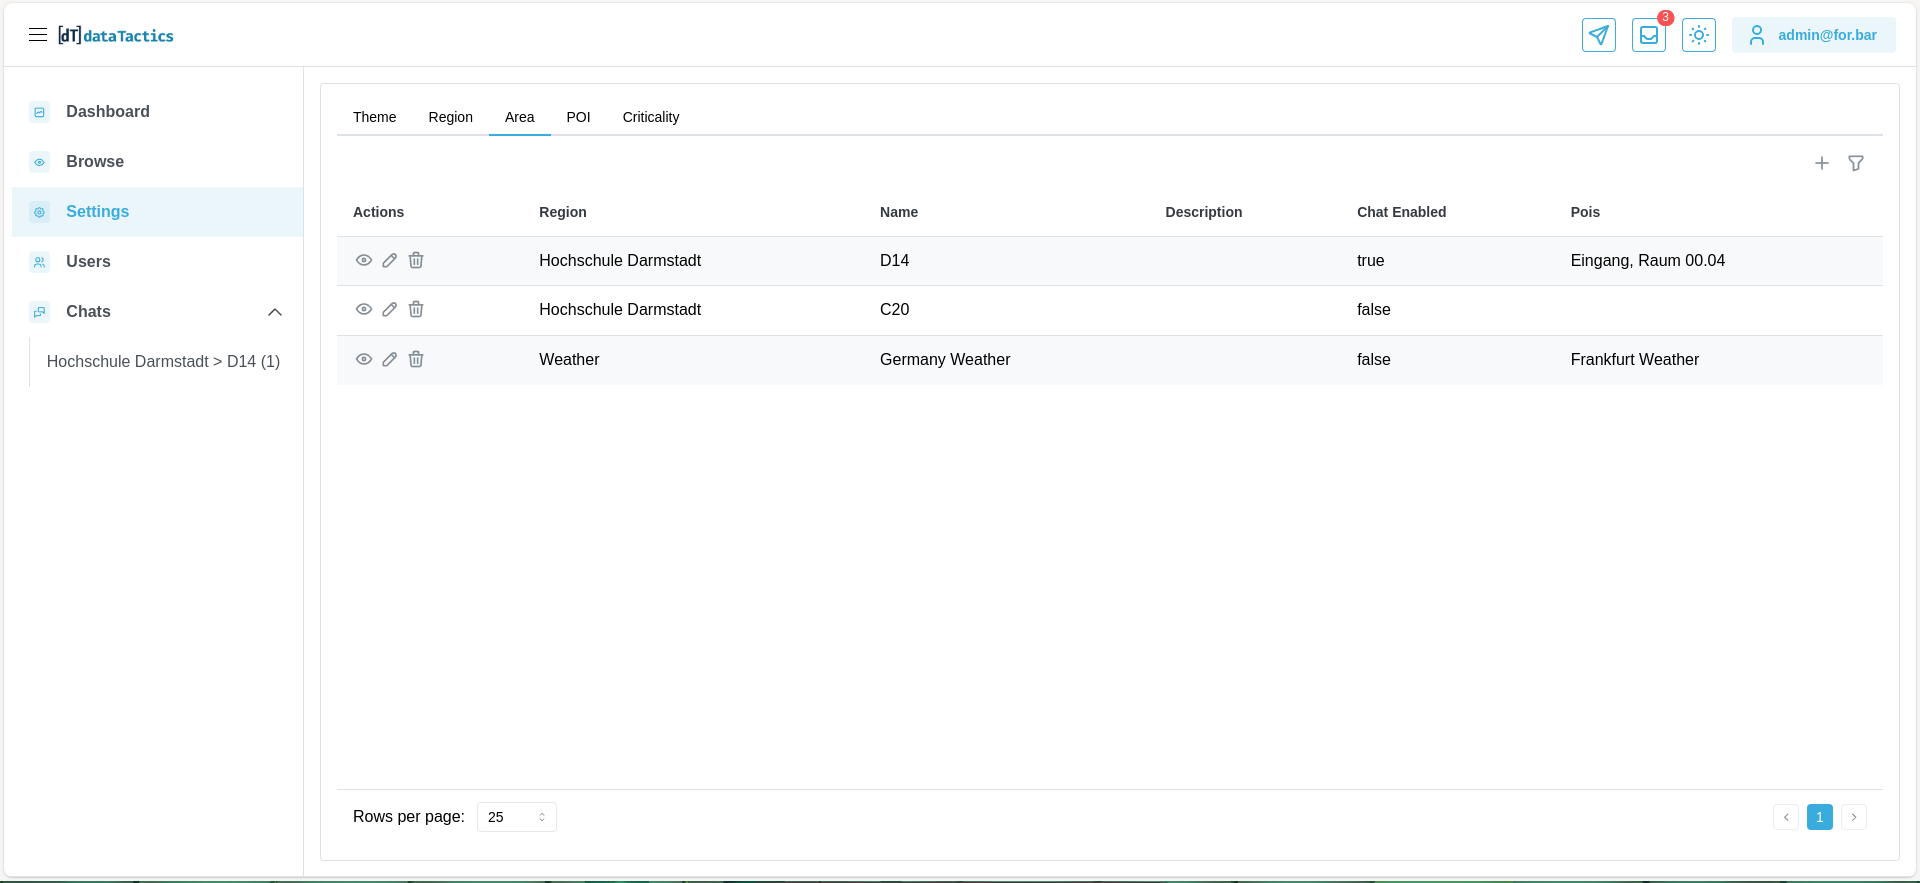
\includegraphics[width=1\textwidth]{gfx/opsedge-settings.png}
    \caption{OpsEdge Settings}
    \label{fig:opsedge_settings}
\end{figure}

\begin{figure}[h]
    \centering
    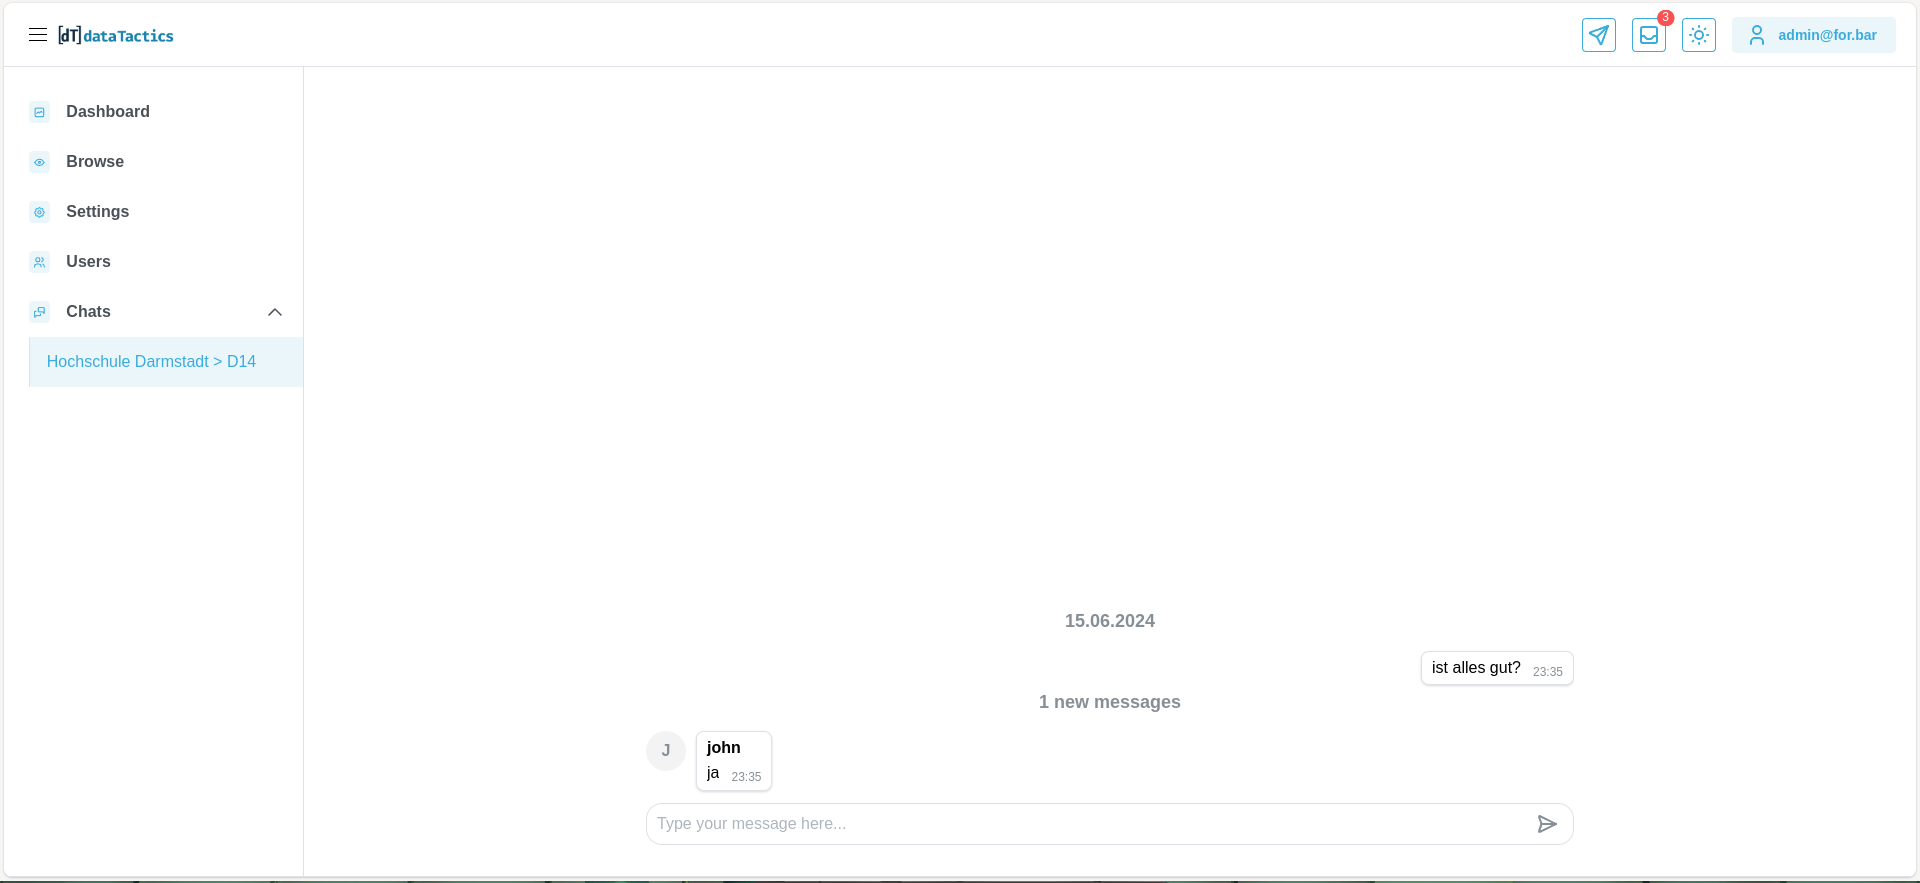
\includegraphics[width=1\textwidth]{gfx/opsedge-chat.png}
    \caption{OpsEdge Chat}
    \label{fig:opsedge_chat}
\end{figure}